\documentclass[10pt,a4paper]{article}
\usepackage[a4paper, total={6.5in, 9in}]{geometry}
\usepackage[latin1]{inputenc}
\usepackage{amsmath}
\usepackage{amsfonts}
\usepackage{amssymb}
\usepackage{mathtools}
\usepackage{graphicx}
\usepackage{float}
\usepackage[usenames, dvipsnames]{color}
\usepackage{fancyhdr}
\usepackage{enumitem}
\usepackage{listings}
\setlength{\headheight}{15.2pt}
\pagestyle{fancy}
\setlength{\parindent}{0em}
\setlength{\parskip}{10pt}
\setlist[enumerate,1]{label=\alph*)}
\setlist[enumerate,2]{label=(\roman*)}
\definecolor{LGray}{gray}{0.9}
\lstset{language=MATLAB, tabsize=2, breaklines=true, postbreak=\mbox{\textcolor{red}{$\hookrightarrow$}\space}, basicstyle=\linespread{0.7}\ttfamily, } 
\newcommand*\diff{\mathop{}\!\mathrm{d}}



\begin{document}
\title{ENGSCI768 A1}
\author{Benjamin Yi}
\rhead{Benjamin Yi - byi649 - 925302651}
\lhead{ENGSCI768 A1}
	
\section*{Question 1}
Note: all functions take an additional optional argument that is used for question 2. \textbf{This additional argument must be left empty when testing question 1}.
 
\newpage
\section*{Question 2}
Hooke-Jeeves:
\begin{figure} [H]
	\centering
	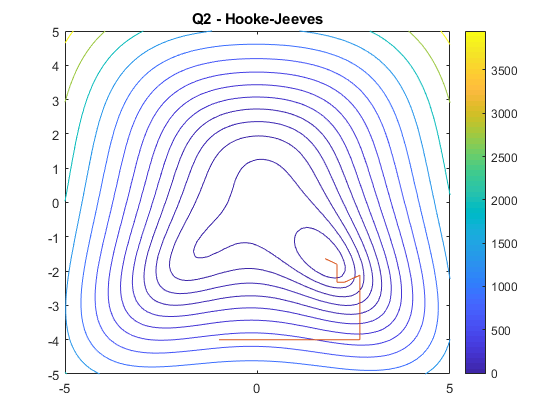
\includegraphics[width=0.7\linewidth]{q2hj}
\end{figure}
Iteration points: \\
Each column is an iteration point, row 1 containing \(x_1\) and row 2 containing \(x_2\).
\begin{figure} [H]
	\centering
	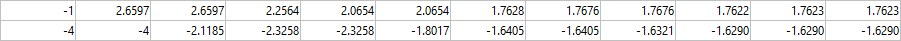
\includegraphics[width=1\linewidth]{q2hjp}
\end{figure}
Objective functions: \\
Each column is an iteration point.
\begin{figure} [H]
	\centering
	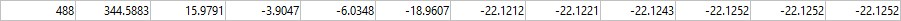
\includegraphics[width=1\linewidth]{q2hjf}
\end{figure}

\newpage
Steepest descent:
\begin{figure} [H]
	\centering
	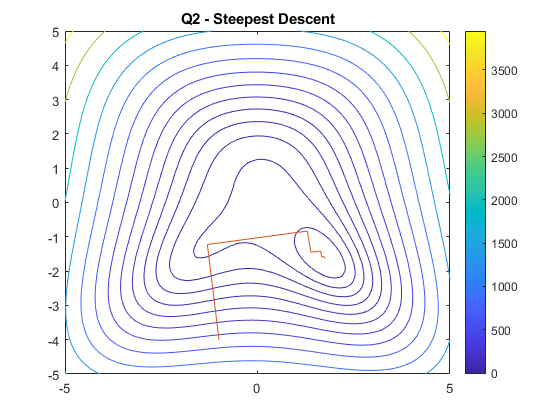
\includegraphics[width=0.7\linewidth]{q2sd}
\end{figure}
Iteration points: \\
Each column is an iteration point, row 1 containing \(x_1\) and row 2 containing \(x_2\).
\begin{figure} [H]
	\centering
	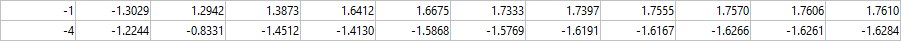
\includegraphics[width=1\linewidth]{q2sdp}
\end{figure}
Gradients: \\
Each column is an iteration point, row 1 is in the direction of \(x_1\) and row 2 is in the direction of \(x_2\).
\begin{figure} [H]
	\centering
	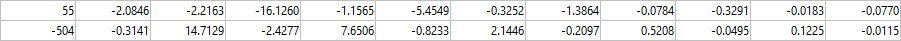
\includegraphics[width=1\linewidth]{q2sdg}
\end{figure}
Objective functions: \\
Each column is an iteration point.
\begin{figure} [H]
	\centering
	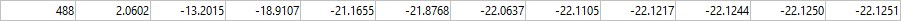
\includegraphics[width=1\linewidth]{q2sdf}
\end{figure}

\newpage
Newton's Method:
\begin{figure} [H]
	\centering
	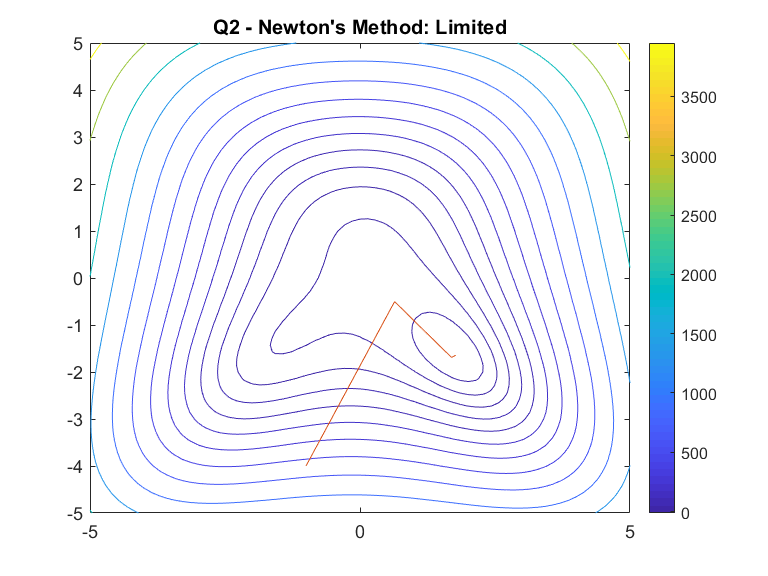
\includegraphics[width=0.7\linewidth]{q2nl}
\end{figure}
Iteration points: \\
Each column is an iteration point, row 1 containing \(x_1\) and row 2 containing \(x_2\).
\begin{figure} [H]
	\centering
	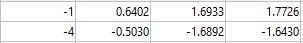
\includegraphics[width=0.7\linewidth]{q2nlp}
\end{figure}
Gradients: \\
Each column is an iteration point, row 1 is in the direction of \(x_1\) and row 2 is in the direction of \(x_2\).
\begin{figure} [H]
	\centering
	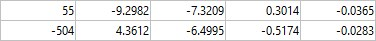
\includegraphics[width=0.7\linewidth]{q2nlg}
\end{figure}
Objective functions: \\
Each column is an iteration point.
\begin{figure} [H]
	\centering
	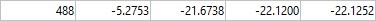
\includegraphics[width=0.7\linewidth]{q2nlf}
\end{figure}

\newpage
Pure Newton's Method:
\begin{figure} [H]
	\centering
	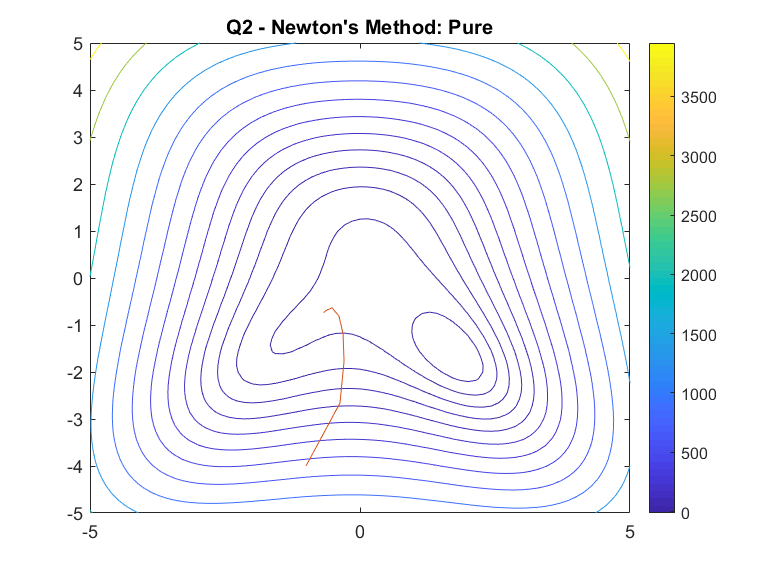
\includegraphics[width=0.7\linewidth]{q2np}
\end{figure}
Pure Newton's method finishes with final objective value = 2.2271. It does not reach the global minima (f = -22.1252), instead finding some other local minima. This is because it does not travel far enough in the first step.
\newpage
\section*{Question 3}
\section*{Question 4}
\begin{enumerate}
	\item
	Sufficient conditions:
	\begin{align}
		\nabla f(x^*) &= 0 \\
		d^TH(x^*)d &> 0
	\end{align}
	Consider (1):
	\begin{align*}
		f(x^*) &= \sum_{k=1}^{n}(p_k \times (y_k - x^*)^2) \\
		\nabla f(x^*) &= \sum_{k=1}^{n}(p_k \times (y_k - x^*)(-2)) = 0 \\
	\end{align*}
	\begin{align*}
		\sum_{k=1}^{n}(p_k \times (y_k - x^*)) &= 0 \\
		\sum_{k=1}^{n}(p_k \times y_k - p_k \times x^*)) &= 0 \\
		\sum_{k=1}^{n}p_k \times y_k &= \sum_{k=1}^{n}p_k \times x^* \\
		x^* &= \sum_{k=1}^{n}(p_k \times y_k) / \sum_{k=1}^{n} p_k \\
		x^* &= \sum_{k=1}^{n}(p_k \times y_k)
	\end{align*}
	Consider (2):
	\begin{equation*}
	H(x^*) = \sum_{k=1}^{n}(2 \times p_k)
	\end{equation*}
	\begin{align*}
		d^TH(x^*)d &> 0 \\
		\sum_{k=1}^{n}(2 \times p_k \times d^2) &> 0 \\
		\sum_{k=1}^{n}(p_k) &> 0
	\end{align*}
	(1) states \(x^*\) is optimal at \(x^* = \sum_{k=1}^{n}(p_k \times y_k)\). (2) is satisfied by the definition of \(p_k\). When \(p_k = \frac{1}{n}\), \(x^*\) is the mean value of \(y_k\).
	\item 
	\begin{align*}
	&\text{ min E}[ \, | Y - x| \, ] \\
	= &\text{ min } \sum_{k=1}^{n} ( p_k \times | y_k - x | ) \\
	= &\text{ min } \sum_{k=1}^{n} ( \frac{1}{n} \times | y_k - x | ) \\
	= &\text{ min } \sum_{k=1}^{n} ( \frac{1}{n} \times \text{max}(y_k - x, -(y_k - x) )
	\end{align*}
	Let \(f(x) = \sum_{k=1}^{n} g_k(x)\) such that \(g_k(x) = \frac{1}{n} \times \text{max}(y_k - x, -(y_k - x)) \). \\ \\
	Then, defining \(d^+, d^-\) as positive and negative direction respectively: 
	\begin{align*}
	g_k'(x; d^+) = -&\frac{1}{n} && \text{if } x < y_k \\
	& \frac{1}{n} && \text{if } x > y_k \\
	& \frac{1}{n} && \text{if } x = y_k
	\end{align*}
	\begin{align*}
	g_k'(x; d^-) = &\hphantom{-}\frac{1}{n} && \text{if } x < y_k \\
	& -\frac{1}{n} && \text{if } x > y_k \\
	& \hphantom{-}\frac{1}{n} && \text{if } x = y_k
	\end{align*}
	From page 52 of lecture notes we have: 
	\begin{equation*}
	f'(x) = \sum_{k=1}^{n} g_k'(x)
	\end{equation*}
	Note that there are 2 possible values for \(g_k'(x)\) depending on the value of \(y_k\) relative to \(x_k\). We denote \(N_{(>)}\) as the number of \(y_k > x\) and \(N_{(<)}, N_{(=)}\) similarly. Then: 
	\begin{align*}
	f'(x; d^+) &= -\frac{1}{n} \times N_{(<)} + \frac{1}{n} \times N_{(>)} + \frac{1}{n} \times N_{(=)} \\
	f'(x; d^-) &= \frac{1}{n} \times N_{(<)} + -\frac{1}{n} \times N_{(>)} + \frac{1}{n} \times N_{(=)}
	\end{align*}
	Point \(x^*\) is at a global minima if \(f'(x^*; d) \geq 0 \, \forall d\) as per page 52 of the lecture notes. We then have two conditions to meet: 
	\begin{align*}
	N_{(>)} + N_{(=)} &\geq N_{(<)} \\
	N_{(<)} + N_{(=)} &\geq N_{(>)}
	\end{align*}
	Re-ordering \(y_k\) such that \(y_1 \leq y_2 \leq \dots \leq y_n\), \(x^*\) is optimal between \([y_a, y_b]\) inclusive, where \(a = \lfloor\frac{n}{2}\rfloor, b = \lceil\frac{n}{2}\rceil\). This is when \(x^*\) has half the \(y_k\) values above it, and half below it.
	
\end{enumerate}

	
\end{document}

